%\documentclass[9pt]{book}
\documentclass[landscape,14pt]{oblivoir}
    \usepackage{a4wide}
    \usepackage{palatino}
    \usepackage{newcent}
    \usepackage{amsmath,amsfonts,amssymb}
	\usepackage{graphics} % for pdf, bitmapped graphics files
	\usepackage{epsfig} % for postscript graphics files
	\usepackage{xcolor}

    \setlength{\parindent}{0mm}
    \setlength{\textheight}{183.0mm}
    \setlength{\oddsidemargin}{-11.0mm}
    \setlength{\textwidth}{243.5mm}
   \setlength{\topmargin}{-16.0mm} 

\begin{document}

    \baselineskip 20pt
    \thispagestyle{empty}

%
%%%%%%%%%%%%%%%%%%%%%%%%%%%%%%%%%%%%%%%%%%%%%%%%%%%%%%%%%%%%%%%%%%%%%%%%%%%%%%%%%
%   Chapter 8
\setcounter{chapter}{7}

\setcounter{section}{0}
%%%%%%%%%%%%%%%%%%%%%%%%%%%%%%%%%%%%%%%%%%%%%%%%%%%%%%%%%%%%%%%%%%%%%%%%%%%%%%%%%
\chapter{Digital Control} 
%
\section{Digitization}
\begin{enumerate}
	\item Most control systems use digital computers (usually microprocessors) to implement the controller. 
	\item Sampler and A/D Converter, D/A Converter and ZOH (Zeroth-Order Holding), and Clock
	\begin{figure}[h]
		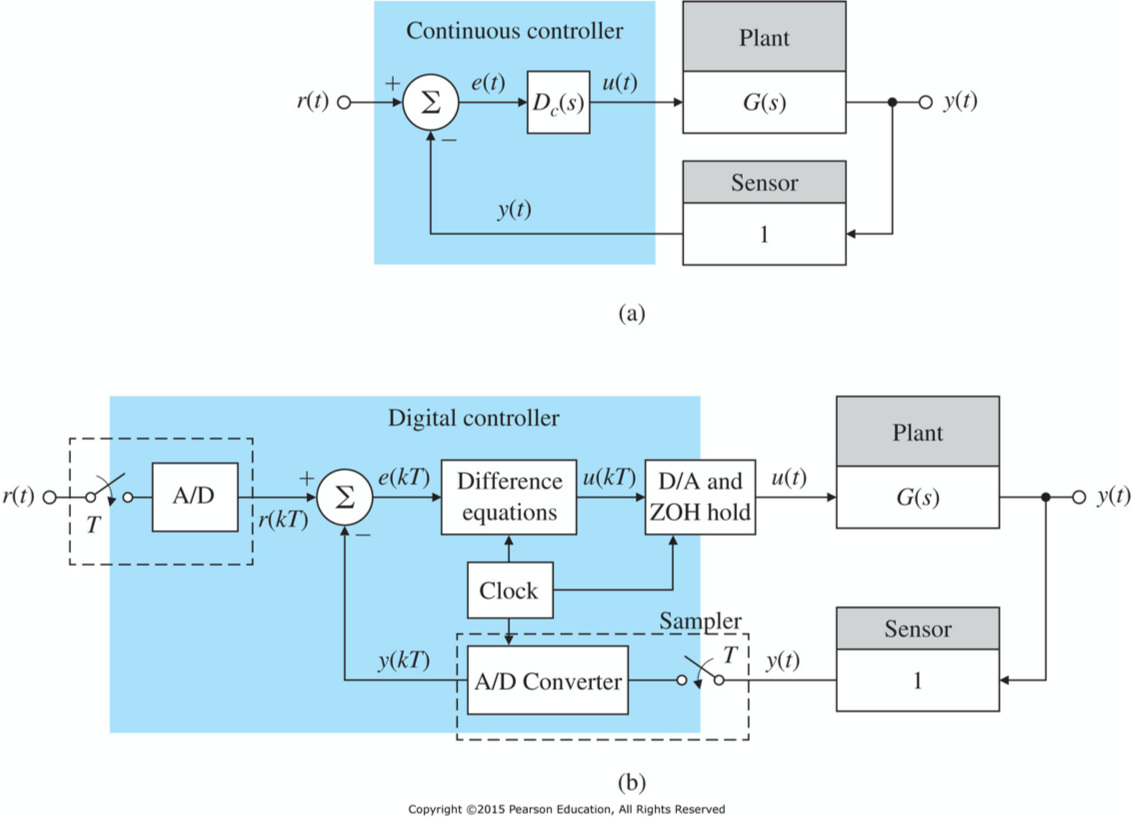
\includegraphics[width=12cm]{./FIG_Franklin/fig8-1.png}
	\end{figure}
%
\newpage
%
	\item The computation of error signal $e(t)$ and the dynamic compensation $D_c(s)$ can all be accomplished in a digital computer. 
	\item Difference equation for discrete-time system $\leftrightarrow$ Differential equation for continuous-time system 
	\item Two basic techniques for finding the difference equations for the digital controller, from $D_c(s)$ to $D_d(z)$ 
	\begin{itemize}
		\item Discrete equivalent - section 8.3 
		\item Discrete design  - section 8.7 
	\end{itemize}
	\item The analog output of the sensor is sampled and converted to a digital number in the analog-to-digital (A/D) converter. (Sampler and ADC)
	\begin{itemize}
		\item Conversion from the continuous analog signal $y(t)$ to the discrete digital samples $y(kT)$ occurs repeatedly at instants of time $T$ apart where $T$ is the sample period [$s$] and $1/T$ is the sample rate [$Hz$].
		\begin{align*}
			y(t) ~~~~ \rightarrow~~~~~y (k) = y(kT) ~~~~\mbox{with} ~~ t = kT  
		\end{align*}
		where $k$ is an integer and $T$ is a fixed value (sample period, or sampling time). 
		\item The sampled signal is $y(kT)$, where $k$ can take on any integer value. 
		\item It is often written simply as $y(k)$. We call this type of variable a discrete signal. 
	\end{itemize}   
%
\newpage
%
	\item The D/A converter changes the digital binary number to an analog voltage, and a zeroth-order hold maintains the same voltage throughout the sample period $T$. (DAC and ZOH)
	\begin{figure}[h]
		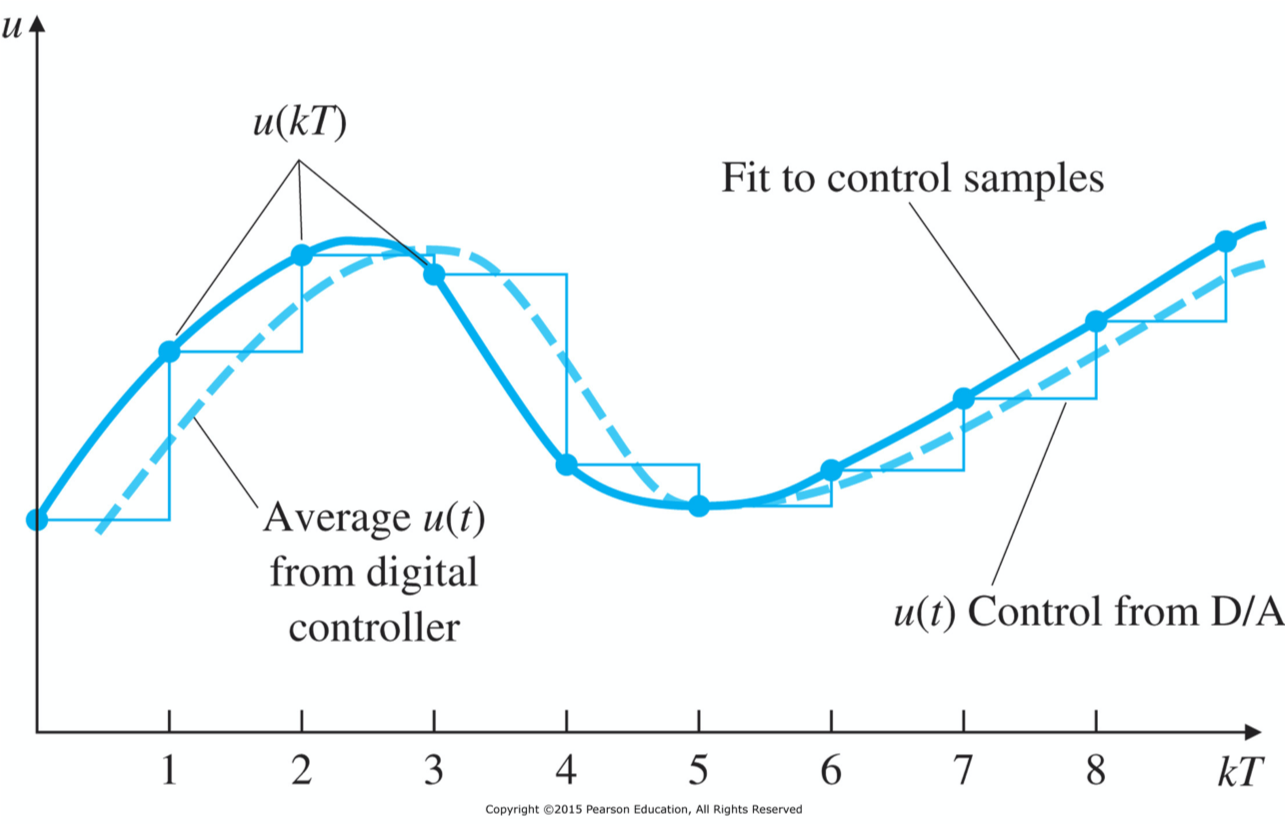
\includegraphics[width=9cm]{./FIG_Franklin/fig8-2.png}
	\end{figure}
	\begin{itemize}
		\item Because each value of $u(kT)$ in Fig. 8.1(b) is held constant until the next value is available from the computer, the continuous value of $u(t)$ consists of steps (see Fig. 8.2) that, on average, are delayed from a fit to $u(kT)$ by $T/2$ as shown in the figure. 
		\item Sample rates should be at least 20 times the bandwidth in order to assure that the digital controller will match the performance of the continuous controller.
		\item If we simply incorporate this $T/2$ delay into a continuous analysis of the system, an excellent prediction results in, especially, for sample rates much slower than 20 times bandwidth.
	\end{itemize}
	\item A system having both discrete and continuous signals is called a `sampled data system'. 
\end{enumerate}
%
%
\newpage
%
\section{Dynamic Analysis of Discrete Systems}
\begin{itemize}
	\item $z$-transform for discrete time systems $\leftrightarrow$ Laplace transform for continuous time systems. 
	\item (8.2.1) $z$-Transform 
	\begin{enumerate}
		\item Laplace transform and its important property 
		\begin{align*}
			\mathcal{L} (f(t))&= F(s) = \int_0^{\infty} f(t) e^{-st} dt 
			&&&
			\mathcal{L}(\dot{f}(t)) &= sF(s) 
		\end{align*}
		where $f(0^+) = 0$
		\item $z$-transform is defined by 
		\begin{align*}
			\mathcal{Z}(f(k)) &= F(z) = \sum_{k=0}^{\infty} f(k) z^{-k}  
			&&&
			\mathcal{Z} (f(k-1)) &=   \sum_{k=0}^{\infty} f(k-1) z^{-k}  
			\\
			&= f(0) + f(1) z^{-1} + f(2) z^{-2} + \cdots
			&&&
			&= f(-1) + f(0) z^{-1} + f(1) z^{-2} + f(2) z^{-3} + \cdots \\
			& &&& &= z^{-1} \left[  f(0) + f(1) z^{-1} + f(2) z^{-2} + \cdots \right] \\ 
			& &&& &= z^{-1} F(z) 
		\end{align*}
		where $f(k)$ is the sampled version of $f(t)$ and $z^{-1}$ represents one sample delay, and $f(-1) = 0$. 
		\item Important property between LT and $z$-transform
		\begin{align*}
			z = e^{sT} ~~~~ \leftrightarrow~~~~ s = \frac{1}{T} \ln z  
		\end{align*}
		\item For example, the general second-order difference equation 
		\begin{align*}
			y(k) = -a_1 y(k-1) - a_2 y(k-2) + b_0 u(k) + b_1 u(k-1) + b_2 u(k-2) 
		\end{align*}
		can be converted from this form to the $z$-transform of the variables $y(k)$ and $u(k)$ by invoking above relations,
		\begin{align*}
			Y(z) = (-a_1 z^{-1} - a_2 z^{-2}) Y(z) + (b_0 + b_1 z^{-1} + b_2 z^{-2}) U(z) 
		\end{align*}
		now we have a discrete transfer function:
		\begin{align*}
			\frac{Y(z)}{U(z)} = \frac{b_0 + b_1 z^{-1} + b_2 z^{-2}}{1 + a_1 z^{-1} + a_2 z^{-2}} 
		\end{align*}
	\end{enumerate}
%
\newpage
%
	\item (8.2.2) $z$-Transform Inversion
	\begin{enumerate}
		\item See the Table 8.1 for understanding between $z$-transform and LT
		\begin{table}[h]
			\begin{tabular}{c||c||c|c} 
				\hline \hline 
				$F(s)$ & $f(kT)$ & $F(z)$ & \\ \hline
				- & 1, $k=0$ and 0, $k \neq 0$ & 1 & \\
				- & 1, $k=k_0$ and 0, $k \neq k_0$ & $z^{-k_0}$ & \\
				$\frac{1}{s}$ & $1(kT)$ & $\frac{z}{z-1}$ & $\frac{1}{1-z^{-1}}$ \\
				$\frac{1}{s^2}$ & $kT$ & $\frac{Tz}{(z-1)^2}$ & $\frac{Tz^{-1}}{(1-z^{-1})^2} $ \\
				$\frac{1}{s+a}$ & $e^{-akT}$ & $\frac{z}{z-e^{-aT}}$ & $\frac{1}{1-e^{-aT}z^{-1}}$ \\
				$\frac{1}{s(s+a)}$ & $1-e^{-akT}$ & $\frac{z(1-e^{-aT})}{(z-1)(z-e^{-aT})}$ & $\frac{z^{-1}(1-e^{-aT})}{(1-z^{-1})(1-e^{-aT} z^{-1})}$ \\
				$\frac{a}{s^2+a^2}$ & $\sin a kT$ & $\frac{z \sin aT}{z^2-(2\cos aT)z +1}$ & $\frac{z^{-1}  \sin aT}{1-(2\cos aT)z^{-1} + z^{-2}}$ \\
				$\frac{s}{s^2+a^2}$ & $\cos a kT$ & $\frac{z(z- \cos aT)}{z^2-(2\cos aT)z +1}$ & $\frac{(1- z^{-1}\cos aT )}{1-(2\cos aT)z^{-1} +z^{-2}}$ \\
				\hline \hline 
			\end{tabular}
		\end{table}
		\item For parts of Table, we have
		\begin{align*}
			\mathcal{Z}(\delta(t)) &= 1  + 0 z^{-1} + 0 z^{-2} + \cdots = 1  \\  
			\mathcal{Z}(\delta(t=k_0T)) &= 0  + 0 z^{-1} +  \cdots + 1 z^{-k_0} + \cdots +  = z^{-k_0}  \\  
			\mathcal{Z}(1(t)) &= 1 + z^{-1} + z^{-2} + \cdots = \frac{1}{1-z^{-1}} = (1-z^{-1})^{-1}  \\
			\mathcal{Z}(e^{-at}) &= 1 + e^{-aT} z^{-1} + e^{-2aT} z^{-2} + \cdots = \frac{1}{1-e^{-aT}z^{-1}} 
		\end{align*}
%
\newpage
%
		\item The differentiator $s$ is transformed into $z$-domain 
		\begin{align*}
			\frac{1}{s} ~~\leftrightarrow~~ \frac{1}{1-z^{-1}}  ~~~~~~~~~~~~
			s ~~\leftrightarrow~~ (1-z^{-1})  
		\end{align*}
		\item $z$-transform of ramp signal $t= kT$ becomes
		\begin{align*}
				\mathcal{Z}(t) &= 0 + Tz^{-1} + 2T z^{-2} + 3T z^{-3} +  \cdots  \\
				&= T[z^{-1} + 2 z^{-2} + 3 z^{-3} +  \cdots]  \\
				z^{-1}\mathcal{Z}(t) &= T[ z^{-2} + 2 z^{-3} + 3 z^{-4} +  \cdots]  \\
				(1-z^{-1}) \mathcal{Z}(t) &=  T[z^{-1} + z^{-2} + z^{-3} +  \cdots] 
				= T \frac{z^{-1}}{1-z^{-1}}   \\
				\mathcal{Z}(t) &=  \frac{Tz^{-1}}{(1-z^{-1})^2}  
		\end{align*}
%
\newpage
%
		\item A $z$-transform inversion technique that has no continuous counterpart is called `long division'. For example, consider a first-order discrete system 
		\begin{align*}
			y(k) = \alpha y(k-1) + u(k) ~~~~\rightarrow~~~~~ \frac{Y(z)}{U(z)} = \frac{1}{1-\alpha z^{-1}}
		\end{align*} 
		For a unit-pulse input, its $z$-transform is 
		\begin{align*}
			U(z) = 1 
		\end{align*}
		so the long division becomes 
		\begin{align*}
			Y(z) &= \frac{1}{1-\alpha z^{-1}} \\
			&= 1 + \alpha z^{-1} + \alpha^2 z^{-2} + \alpha^3 z^{-3}  \cdots  		
		\end{align*}
		We see that the sampled time history of $y$ is
		\begin{align*}
			y(0) &= 1 &&& y(1) &= \alpha &&& y(2) &= \alpha^2 &&& y(3) &= \alpha^3 ~~~~\cdots 
		\end{align*}
	\end{enumerate}
%
\newpage
%
	\item (8.2.3) Relationship between $s$ and $z$ 
	\begin{enumerate}
		\item Consider the continuous signal of 
		\begin{align*}
			f(t) &= e^{-at} ~~~~~ t >0 \\ 
			F(s) &= \int_0^{\infty} f(t) e^{-st} dt  = \int_0^{\infty} e^{-(s+a)t} dt = 
			\frac{1}{s+a}
		\end{align*}
		and it corresponds to a pole $s=-a$. 
		\item Consider the discrete signal of 
		\begin{align*}
			f(kT) &= e^{-akT}  \\  
			F(z) &= \sum_{k=0}^{\infty} f(kT) z^{-k}   = 1 + e^{-aT} z^{-1} + e^{-2aT} z^{-2} + e^{-3aT} z^{-3} +  \cdots ~~~~\mbox{무한등비급수} \\
			&= \frac{\mbox{초기치}}{1- \mbox{공비}} = \frac{1}{1-e^{-aT}z^{-1}} = \frac{z}{z-e^{-aT}}
		\end{align*}
		and it corresponds to a pole $z=e^{-aT}$. 
		\item The equivalent characteristics in the $z$-plane are related to those in the $s$-plane by the expression
		\begin{align*}
			z &= e^{sT} = e^{-aT +jbT} = e^{-aT} (\cos bT + j \sin b) \\
			&= e^{-\sigma T} (\cos \omega_d T + j \sin \omega_d T ) \\
			&= e^{-\zeta \omega_n T} (\cos \omega_n \sqrt{1-\zeta^2} T + j \sin \omega_n \sqrt{1-\zeta^2} T )
		\end{align*}
		where $T$ is the sample period, and $s = -\sigma  + j \omega_d = -\zeta \omega_n + j \omega_n \sqrt{1-\zeta^2} $
\newpage
%
		\item See Fig. 8.4, and it shows the mapping of lines of constant damping $\zeta$ and natural frequency $\omega_n$ from $s$-plane to the upper half of the $z$-plane, using $z = e^{sT}$. 
		\begin{figure}[h]
			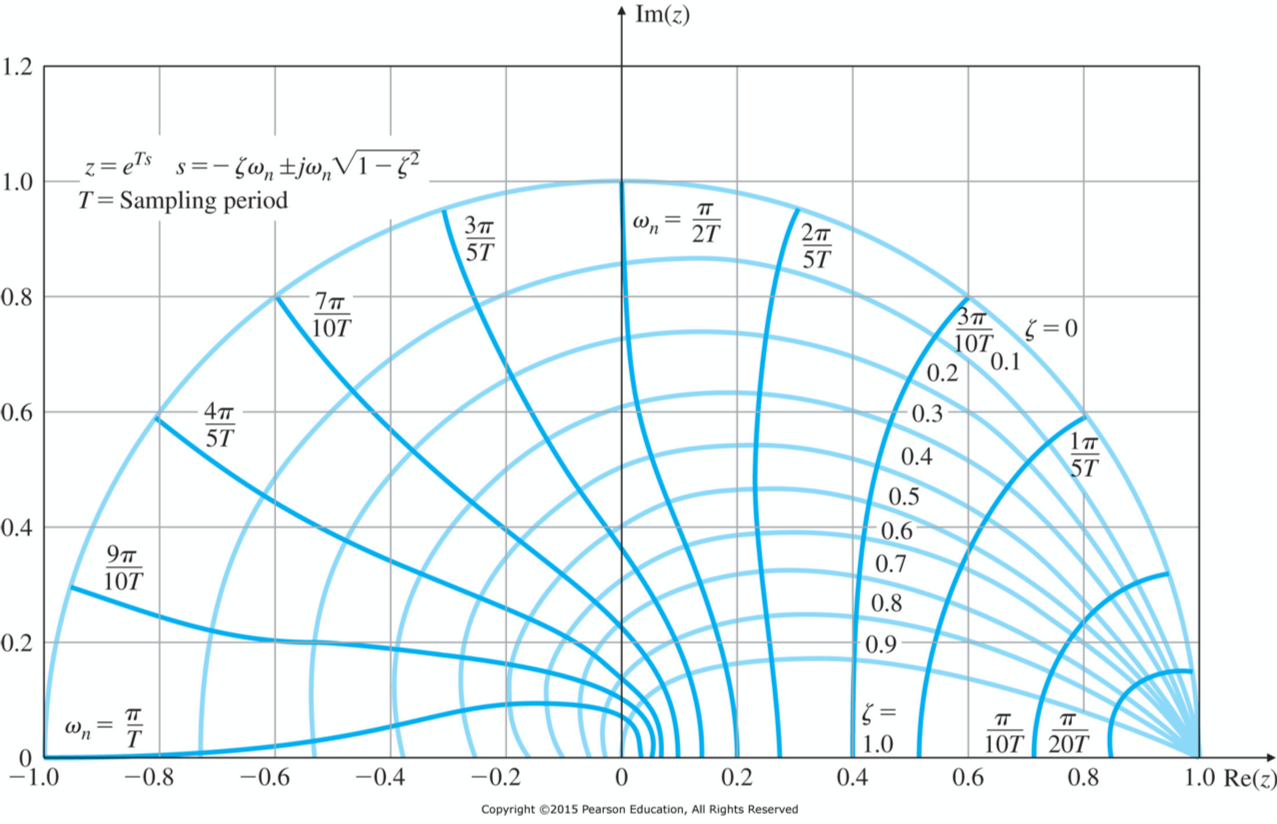
\includegraphics[width=10cm]{./FIG_Franklin/fig8-4.png}
		\end{figure}
		\begin{enumerate}
			\item The stability boundary $s= 0 \pm j\omega$ becomes the unit circle $|z| =1$ in the $z$-plane; inside the unit circle is stable, outside is unstable
			\item The small vicinity around $z=+1$ in the $z$-plane is essentially identical to the vicinity around the origin $s=0$, in the $s$-plane.
			\item The $z$-plane locations give response information normalized to the sample rate rather than to time as in the $s$-plane. 
			\item The negative real $z$-axis always represents a frequency of $\omega_s/2$, where $\omega_s = 2\pi/T = $ circular sample rate in radians per second. 
			\item Vertical lines in the left half of the $s$-plane (the constant real part of $s$) map into \emph{circles} within the unit circle of the $z$-plane 
			\item Horizontal lines in the $s$-plane (the constant imaginary part of $s$) map into \emph{radial lines} in the $z$-plane. 
			\item Frequencies greater than $\omega_s/2$, called the Nyquist frequency, appear in the $z$-plane on the top of corresponding lower frequencies because of the circular characteristics of $e^{sT}$. This overlap is called \emph{aliasing} or folding.  
		\end{enumerate} 
		\item As a result, it is necessary to sample at least twice as fast as a signal's highest frequency component in order to represent that signal with the samples. 
		\item The figure sketches time responses that would result from poles at the indicated locations.
		\begin{figure}[h]
			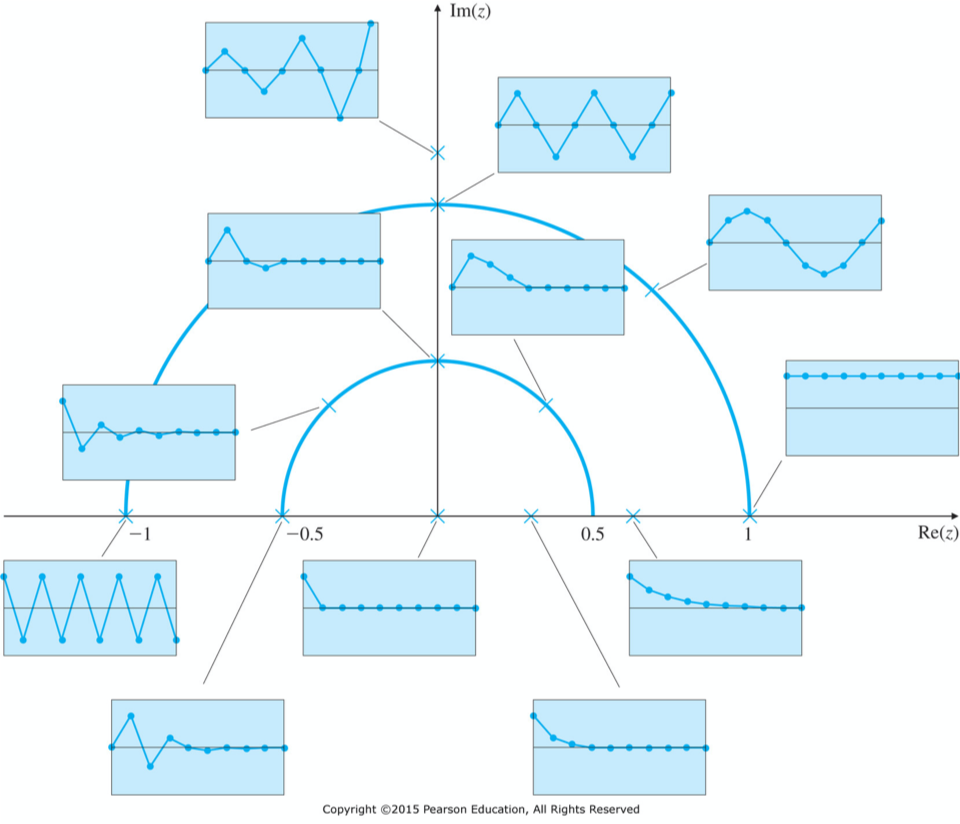
\includegraphics[width=14cm]{./FIG_Franklin/fig8-5.png}
		\end{figure}
	\end{enumerate}
%
\newpage
%
	\item (8.2.4) Final Value Theorem 
	\begin{enumerate}
		\item Discrete final value theorem is 
		\begin{align*}
			\lim_{t \rightarrow \infty} x(t) = x_{ss} &= \lim_{s \rightarrow 0} sX(s) &&&
			\lim_{k \rightarrow \infty} x(k) = x_{ss} &= \lim_{z \rightarrow 1} (1-z^{-1}) X(z) 
		\end{align*}
		if all the poles of $(1-z^{-1}) X(z)$ are inside the unit circle. 
		\item For example, to find the DC gain of the TF
		\begin{align*}
			G(z) = \frac{X(z)}{U(z)} = \frac{0.58(1+z)}{z+0.16} 
		\end{align*}
		we let $u(k) =1 $ for $k \geq 0$, so that 
		\begin{align*}
			U(z) = \frac{1}{1-z^{-1}}
		\end{align*}
		and 
		\begin{align*}
			X(z) = \frac{0.58(1+z)}{(1-z^{-1})(z+0.16)}
		\end{align*}
		Applying the final value theorem yields 
		\begin{align*}
			x_{ss} &= \lim_{z \rightarrow 1} (1-z^{-1}) X(z) = \frac{0.58 \cdot 2}{1+0.16} = 1
		\end{align*}
		so the DC gain of $G(z)$ is unity. 
	\end{enumerate}
\end{itemize}
%
%
\newpage
%
\section{Design using Discrete Equivalents}
\begin{itemize}
	\item It is important to remember that how to convert $D_c(s)$ into $D_d(z)$ is approximation; there is no exact solution for all possible inputs because $D_c(s)$ responds to the complete time history of $e(t)$, whereas $D_d(z)$ has access to only the samples $e(kT)$. 
	\item (8.3.1) Tustin's Method
	\begin{enumerate}
		\item Tustin's method is a digitization technique that approaches the problem as one of numerical integration. Suppose 
		\begin{align*}
			\frac{U(s)}{E(s)}  = D_c(s) = \frac{1}{s} 
		\end{align*}
		which is integration. Therefore, it is corresponding to the \emph{trapezoidal integration} as follows:
		\begin{align*}
			u(kT) &= \int_{0}^{kT-T} e(t) dt + \int_{kT -T}^{kT} e(t) dt \\
			&= u(kT-T) + \mbox{area under $e(t)$ over last period, $T$},  \\
			u(k) &= u(k-1) + T \frac{[e(k-1)+e(k)]}{2}
		\end{align*}
		where $T$ is the sample period. 
		\begin{figure}[h] 
			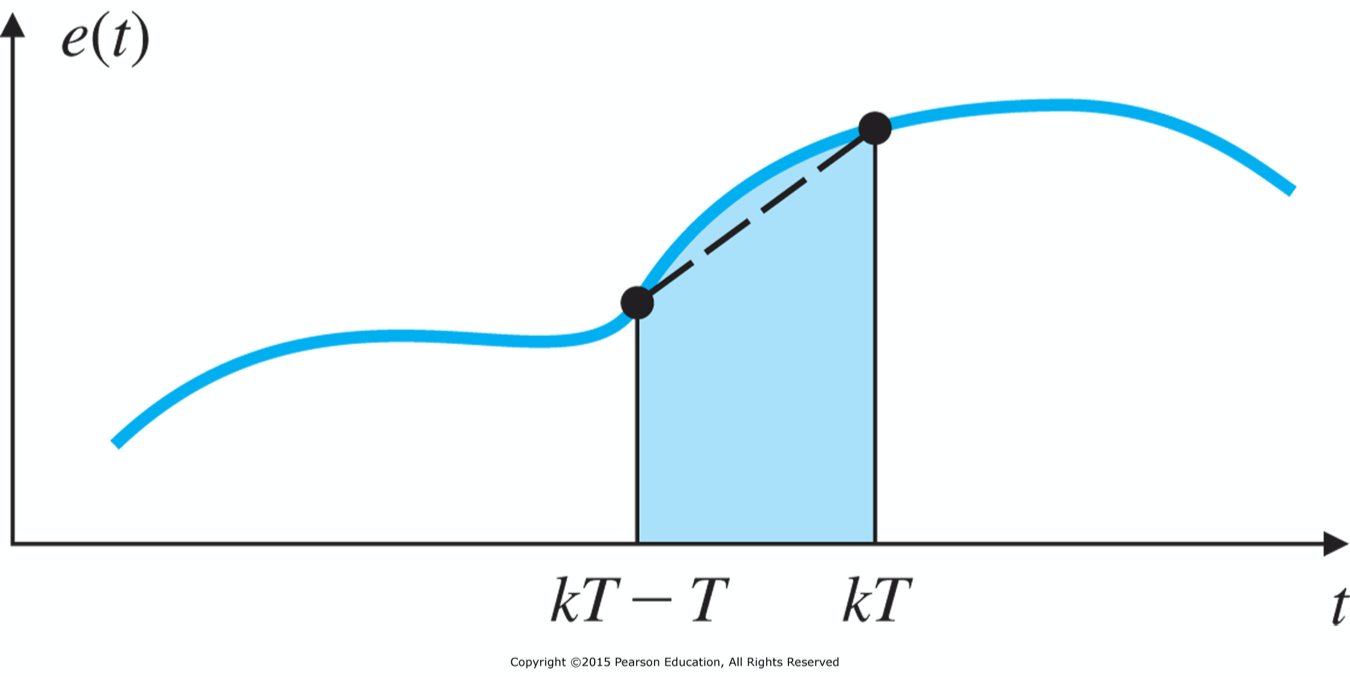
\includegraphics[width=6cm]{./FIG_Franklin/fig8-7.png}
		\end{figure}
		\item Taking $z$-transform, 
		\begin{align*}
			\frac{U(z)}{E(z)} = \frac{T}{2} \frac{1+z^{-1}}{1-z^{-1}} = \frac{1}{\frac{2}{T} \frac{1-z^{-1}}{1+z^{-1}} }
		\end{align*}
		\item In fact, the Tustin's method approximates $z = e^{sT}$ as follows:
		\begin{align*}
			s \approx  \frac{2}{T} \frac{1-z^{-1}}{1+z^{-1}}
		\end{align*}
		where it can be derived from the Taylor's series expansions as follows:
		\begin{align*}
			z &= e^{sT} = \frac{e^{\frac{sT}{2}}}{e^{-\frac{sT}{2}}} 
			= \frac{1 + \frac{sT}{2} + \frac{s^2T^2}{2^2} + \cdots}{1 - \frac{sT}{2} + \frac{s^2T^2}{2^2} - \cdots} \approx  \frac{1 + \frac{sT}{2}}{1 - \frac{sT}{2}}  = \frac{2+sT}{2-sT} 
			~~~~~\rightarrow~~~~~ s \approx  \frac{2}{T} \frac{z-1}{z+1} = \frac{2}{T} \frac{1-z^{-1}}{1+z^{-1}}
		\end{align*}
		\item For $D_c(s) = \frac{a}{s+a}$ as an example, we have 
		\begin{align*}
			D_d(z) &= \frac{U(z)}{E(z)} = \frac{a}{\frac{2}{T} \frac{1-z^{-1}}{1+z^{-1}}+a} = \frac{aT(1+z^{-1})}{2(1-z^{-1}) + aT (1+z^{-1})} = \frac{aT(1+z^{-1})}{(2+aT) - (2-aT)z^{-1}} \\
			(2+aT) u(k) - (2-aT) u(k-1) &= aT [ e(k) + e(k-1) ]  \\
			\therefore~~~~~
			u(k) &= \frac{(2-aT)}{(2+aT)} u(k-1) + \frac{aT}{(2+aT)} [ e(k) + e(k-1) ] 
		\end{align*}
%
\newpage
%
		\item (Example 8.1) Determine the difference equation with a sample rate of 25 times bandwidth using Tustin's approximation. 
		\begin{align*}
			D_c(s) = 10 \frac{s/2+1}{s/10+1}
		\end{align*}
		Since the bandwidth is approximately $\omega_{bd} = 10[rad/s]$, the sampling rate should be
		\begin{align*}
			\omega_s = 25 \times \omega_{bd} = 250 [rad/s] ~~~~ \rightarrow~~~~~ f_s = \frac{\omega_s}{2\pi} \approx 40[Hz] ~~~~\rightarrow~~~~ T = \frac{1}{f_s} = \frac{1}{40} = 0.025[s]
		\end{align*}
		The discrete TF can be obtained as 
		\begin{align*}
			D_d(z) &= 10 \frac{\frac{1}{T} \frac{1-z^{-1}}{1+z^{-1}}+1}{\frac{1}{5T} \frac{1-z^{-1}}{1+z^{-1}}+1} =  10 \frac{5(1-z^{-1})+ 5T(1+z^{-1})}{(1-z^{-1})+ 5T(1+z^{-1})} \\
			&= 50 \frac{(1+T) - (1-T)z^{-1}}{(1+5T) - (1-5T)z^{-1}} 
			= 50 \frac{1.025 - 0.975z^{-1}}{1.125 - 0.875z^{-1}} 
			= \frac{45.556 - 43.333 z^{-1}}{1 - 0.778z^{-1}}
		\end{align*}
		Finally, the difference equation is 
		\begin{align*}
			u(k) &= 0.778 u(k-1) + 45.556 [ e(k) -  0.951 e(k-1) ]
		\end{align*}
%
\newpage
%
		\begin{figure}[h]
			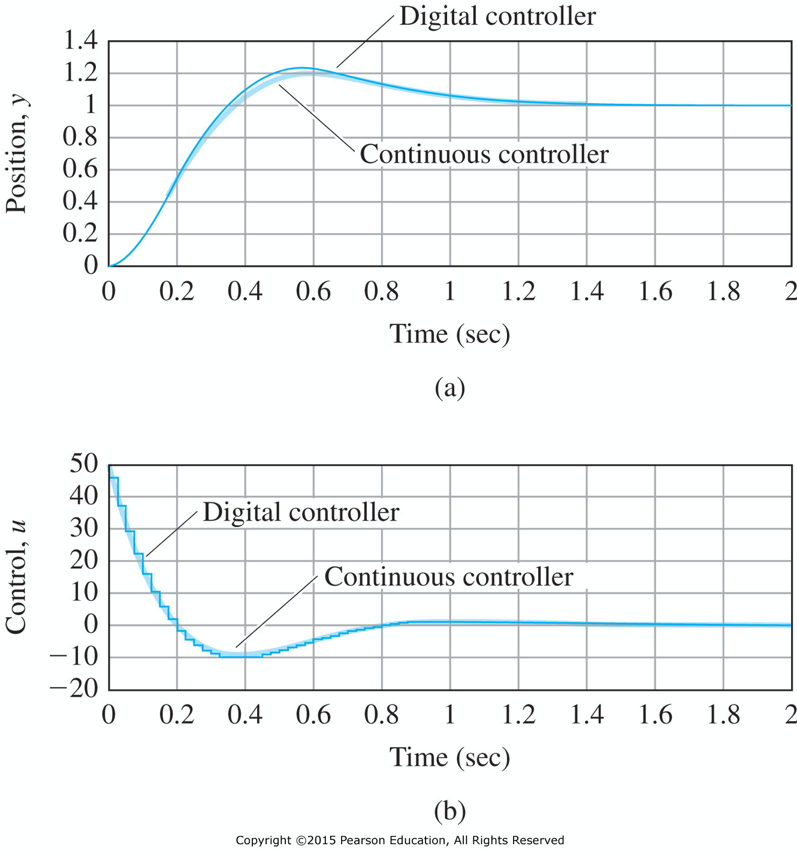
\includegraphics[width=12cm]{./FIG_Franklin/fig8-9.png}
		\end{figure}
	\end{enumerate}
%
\newpage
%
	\item (8.3.2) Zeroth-Order Hold (ZOH) Method 
	\begin{enumerate}
		\item Tustin's method essentially assumed that the input to the controller varied linearly early between the past sample  and the current sample. 
		\item Another assumption is that the input to the controller remains constant throughout the sample period.  $\rightarrow$ ZOH 
		\item One input sample produces a square pulse of height $e(k)$ that lasts for one sample period $T$. 
		\item For a constant positive step input, $e(k)$, at time $k$, $E(s) = e(k)/s$, so the result would be
		\begin{align*}
			D_d(z) = \mathcal{Z} \left( \frac{D_c(s)}{s} \right)
		\end{align*}
		Furthermore, a constant negative step, one cycle delayed, would be 
		\begin{align*}
			D_d(z) = z^{-1} \mathcal{Z} \left( \frac{D_c(s)}{s} \right)
		\end{align*}
		Therefore, the discrete TF for the square pulse is 
		\begin{align*}
			D_d(z) = (1-z^{-1}) \mathcal{Z} \left( \frac{D_c(s)}{s} \right)
		\end{align*}
%
\newpage
%
		\item (Example 8.2) Determine the difference equation with a sample period $T=0.025[s]$ using ZOH approximation. 
		\begin{align*}
			D_c(s) = 10 \frac{s/2+1}{s/10+1} = 10 \frac{5s+10}{s+10}
		\end{align*}
		The discrete TF using ZOH  is 
		\begin{align*}
			D_d(z) = 10 (1-z^{-1}) \mathcal{Z} \left( \frac{5s+10}{s(s+10)} \right)
			&= 10 (1-z^{-1}) \mathcal{Z} \left(  \frac{5}{s+10} + \frac{10}{s(s+10)} \right) \\
			&= 10 (1-z^{-1})  \left( \frac{5}{1-e^{-0.25}z^{-1}} + \frac{z^{-1}(1-e^{-0.25})}{(1-z^{-1})(1-e^{-0.25}z^{-1})} \right) \\
			&=  10 (1-z^{-1})  \left(  \frac{5(1-z^{-1}) + z^{-1}(1-e^{-0.25})}{(1-z^{-1})(1-e^{-0.25}z^{-1})} \right) \\
			&=   \frac{50 - 47.79z^{-1}}{1 - 0.779z^{-1}} 
		\end{align*}
	where $\mathcal{Z} \left\{ \frac{1}{s+10} \right\} = \frac{1}{1-e^{-10T}z^{-1}}$ with  $e^{-10T} = e^{-0.25}=0.779$. Or, 
		\begin{align*}
			D_d(z) = 10 (1-z^{-1}) \mathcal{Z} \left( \frac{5s+10}{s(s+10)} \right)
			&= 10 (1-z^{-1}) \mathcal{Z} \left(  \frac{1}{s} + \frac{4}{s+10} \right) \\
			&= 10 (1-z^{-1})  \left( \frac{1}{1-z^{-1}} + \frac{4}{1-e^{-0.25}z^{-1}} \right) \\
			&=  10 (1-z^{-1})  \left(  \frac{(1-e^{-0.25}z^{-1})+ 4(1-z^{-1})}{(1-z^{-1})(1-e^{-0.25}z^{-1})} \right) \\
			&=   \frac{50 - 47.79z^{-1}}{1 - 0.779z^{-1}} 
		\end{align*}
		Finally, the difference equation is 
		\begin{align*}
			u(k) &= 0.779 u(k-1) + 50 e(k) - 47.79 e(k-1) \\
			&= 0.779 u(k-1) + 50 [ e(k) -  0.956 e(k-1) ]
		\end{align*}
		\begin{figure}[h]
			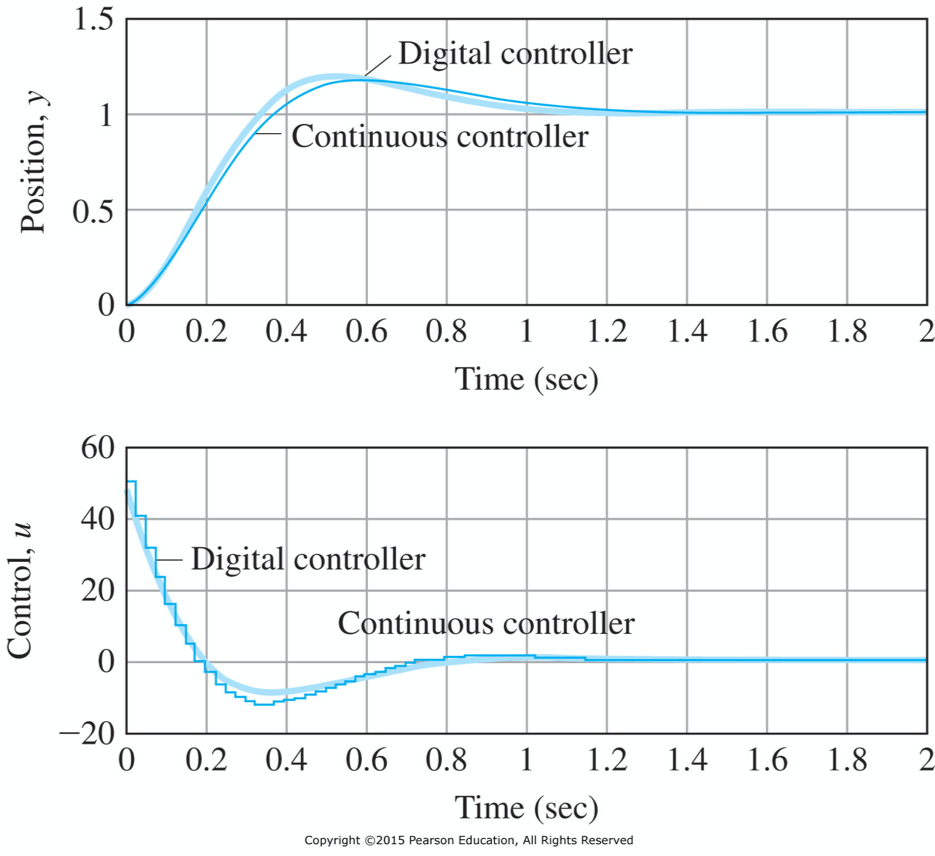
\includegraphics[width=12cm]{./FIG_Franklin/fig8-10.png}
		\end{figure}
	\end{enumerate}
%
\newpage
%
	\item (8.3.3) Matched Pole-Zero (MPZ) Method 
	\begin{enumerate}
		\item Another digitization method, called the matched pole-zero (MPZ) method, is suggested by matching the poles and zeros between $s$ and $z$ planes, using $z = e^{sT}$. 
		\item Because physical systems often have more poles than zeros, it is useful to arbitrarily add zeros at $z=-1$, resulting in a $(1+z^{-1})$ term in $D_d(z)$.
		\begin{enumerate}
			\item Map poles and zeros according to the relation $z = e^{sT}$
			\item If the numerator is of lower order than the denominator, add powers of $(1+z^{-1})$ to the numerator until numerator and denominator are of equal order.
			\item Set the DC or low frequency gain of $D_d(z)$ equal to that of $D_c(s)$.
		\end{enumerate}
		\item For example, the MPZ approximation  
		\begin{align*}
			D_c(s) &= K_c \frac{s+a}{s+b} &&& D_d(z) &= K_d \frac{1-e^{-aT}z^{-1}}{1-e^{-bT}z^{-1}}
		\end{align*}
		where $K_d$ is found by the DC-gain 
		\begin{align*}
			\lim_{s \rightarrow 0} D_c(s) = K_c \frac{a}{b} ~~~~\rightleftarrows~~~~~ 
			\lim_{z \rightarrow 1} D_d(z) = K_d \frac{1-e^{-aT}}{1-e^{-bT}} 
		\end{align*} 
		Thus the result is
		\begin{align*}
			K_d = K_c \frac{a}{b} \left( \frac{1-e^{-bT}}{1-e^{-aT}} \right) 
		\end{align*}
%
\newpage
%
		\item As another example, the MPZ approximation  
		\begin{align*}
			D_c(s) &= K_c \frac{s+a}{s(s+b)} &&& D_d(z) &= K_d \frac{(1+z^{-1})(1-e^{-aT}z^{-1})}{(1-z^{-1})(1-e^{-bT}z^{-1})}
		\end{align*}
		where $K_d$ is found by the DC-gain \emph{by deleting the pure integration term} both sides
		\begin{align*}
			\lim_{s \rightarrow 0} sD_c(s) = K_c \frac{a}{b} ~~~~\rightleftarrows~~~~~ 
			\lim_{z \rightarrow 1} (z-1)D_d(z) = K_d \frac{2(1-e^{-aT})}{1-e^{-bT}} 
		\end{align*} 
		The result is
		\begin{align*}
			K_d = K_c \frac{a}{2b} \left( \frac{1-e^{-bT}}{1-e^{-aT}} \right) 
		\end{align*}
%
\newpage
%
		\item (Example 8.3) Design a digital controller to have a closed-loop natural frequency $\omega_n = 0.3$ and a damping ratio $\zeta = 0.7$, another real pole at $s=-1.58$, using MPZ digitization
		\begin{align*}
			G(s) = \frac{1}{s^2}
		\end{align*}
		Let us assume that the lead compensator is used
		\begin{align*}
			D_c(s) = K_c \frac{s+b}{s+a} 
		\end{align*}
		Then, we have the characteristic equation
		\begin{align*}
			1+G(s) D_c(s) &= 1 + K_c \frac{s+b}{s^2(s+a)}  = s^3 + as^2 + K_c s + K_c b \\
			\alpha_c(s) &= (s^2 + 0.42s + 0.09)(s+1.58) = s^3 + 2s^2 + 0.7536s + 0.1422
		\end{align*}
	    with $a=2$, $b=0.19$, and $K_c = 0.7536$. Now we have the lead compensator: 
		\begin{align*}
			D_c(s) = 0.7536 \frac{s+0.19}{s+2} ~~~~\rightarrow~~~~
			D_c(s) = 0.81 \frac{s+0.2}{s+2}
		\end{align*}
		Let us determine the sampling rate and sampling period as follows:
		\begin{align*}
			\omega_s = 0.3 \times 20 = 6 [rad/s]~~~~\rightarrow~~~~
			f_s = \frac{\omega_s}{2\pi} \approx 1 [Hz]~~~\rightarrow~~~~ T = 1[s]
		\end{align*}
		The MPZ digitization yields 
		\begin{align*}
			D_d(z) = K_d \frac{1-e^{-0.2}z^{-1}}{1-e^{-2}z^{-1}} = K_d  \frac{1-0.818z^{-1}}{1-0.135z^{-1}} 
		\end{align*}
		where the final value theorem gives 
		\begin{align*}
			0.81 \frac{0.2}{2}  = K_d \frac{1-0.818}{1-0.135} ~~~~\rightarrow~~~~K_d = 0.385
		\end{align*}
		The difference equation becomes
		\begin{align*}
			u(k) = 0.135u(k-1) + 0.385 [e(k) - 0.818 e(k-1)] 
		\end{align*}
		For the step responses, 
		\begin{figure}[h]
			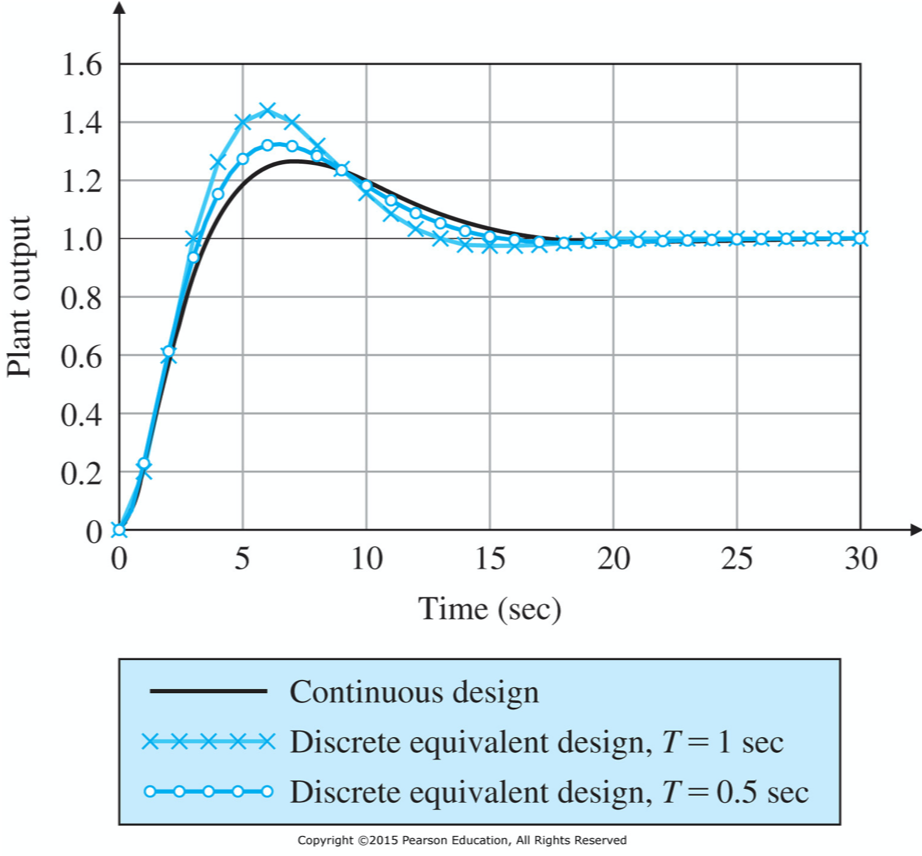
\includegraphics[width=8cm]{./FIG_Franklin/fig8-14.png}
		\end{figure}
	\end{enumerate}
%
\newpage
%
	\item (8.3.4) Modified Matched Pole-Zero (MMPZ) Method 
	\begin{enumerate}
		\item Modify Step 2 in the MPZ so that the numerator is of lower order than denominator by 1. For example, if
		\begin{align*}
			D_c(s) = K_c \frac{s+a}{s(s+b)}
		\end{align*}
		we skip Step 2 to get 
		\begin{align*}
			D_d(z) = K_d \frac{z^{-1}(1-e^{-aT}z^{-1})}{(1-z^{-1})(1-e^{-bT}z^{-1})} ~~~~~~\mbox{where}~~ K_d = K_c \frac{a}{b} \left( \frac{1-e^{-bT}}{1-e^{-aT}} \right) 
		\end{align*}
		We can see the difference equation as follow:
		\begin{align*}
			u(k) = (1+e^{-bT})u(k-1) - e^{-bT} u(k-2) + K_d [ e(k-1) - e^{-aT} e(k-2) ] 
		\end{align*}
		where it makes use of $e(k-1)$ that are one cycle old, not $e(k)$. 
	\end{enumerate}
%
\newpage
%
	\item (8.3.5) Comparison of Digital Approximation Methods 
	\begin{enumerate}
		\item Let us compare four approximation methods with the sampling rate 
		\begin{align*}
			D_c(s) = \frac{5}{s+5}
		\end{align*}
		\item Tustin's method
		\begin{align*}
			D_d(z) &= \frac{5}{\frac{2}{T} \frac{1-z^{-1}}{1+z^{-1}} +5} = \frac{5T(1+z^{-1})}{2(1-z^{-1}) +5T(1+z^{-1})} = \frac{5T + 5T z^{-1}}{ (2+5T) - (2-5T)z^{-1}} \\
			&= \left( \frac{5T}{2+5T} \right) \frac{ 1+ z^{-1} } { 1 - \left( \frac{2-5T}{2+5T} \right) z^{-1}} 
		\end{align*}
		\item ZOH 
		\begin{align*}
			D_d(z) &= (1-z^{-1}) \mathcal{Z} \left( \frac{D_c(s)}{s} \right) =  (1-z^{-1}) \mathcal{Z} \left( \frac{5}{s(s+5)} \right) =(1-z^{-1})  \frac{(1-e^{-5T})z^{-1}}{(1-z^{-1})(1-e^{-5T}z^{-1})} \\
			&= (1-e^{-5T}) \frac{z^{-1}}{1-e^{-5T}z^{-1}} 
		\end{align*}
		\item MPZ 
		\begin{align*}
			D_d(z) &= K_d \frac{(1+z^{-1})}{1-e^{-5T}z^{-1}} ~~~~\mbox{where}~~ K_d \frac{2}{1-e^{-5T}} = 1 \\
			&= \left( \frac{1-e^{-5T}}{2} \right)  \frac{1+z^{-1}}{1-e^{-5T}z^{-1}}  
		\end{align*}
		\item MMPZ
		\begin{align*}
			D_d(z) &= K_d \frac{z^{-1}}{1-e^{-5T}z^{-1}} ~~~~\mbox{where}~~ K_d \frac{1}{1-e^{-5T}} = 1 \\
			&= (1-e^{-5T}) \frac{z^{-1}}{1-e^{-5T}z^{-1}} 
		\end{align*}
		\item It is noted that Tustin and MPZ bring the similar structures each other, while ZOH and MMPZ show the similar structures, as shown in Table 8.2 
		\item Tustin and MPZ methods show a notch at $\omega_s/2$ because of their zero at $z=-1$ from $1+z^{-1}$ term. 
		\begin{figure}[h]
			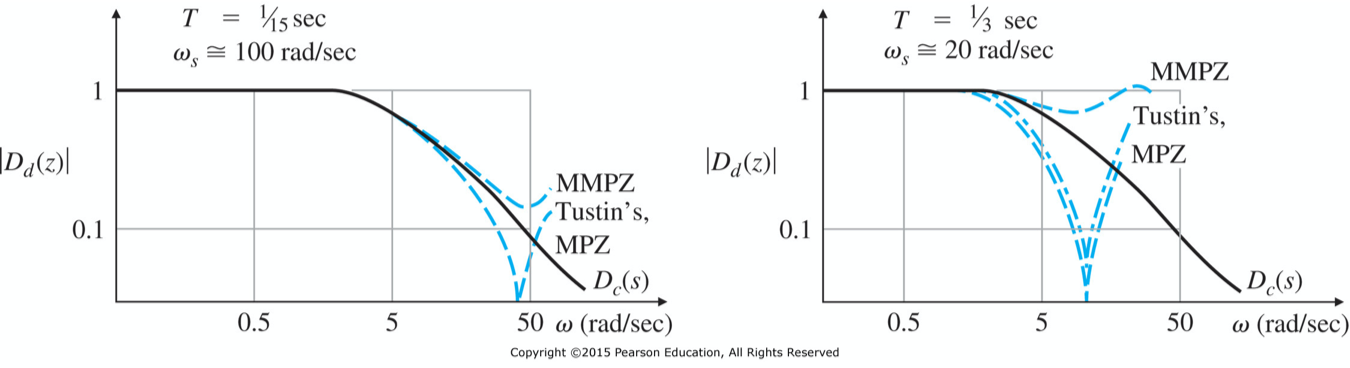
\includegraphics[width=16cm]{./FIG_Franklin/fig8-15.png}
		\end{figure}
	\end{enumerate}
%
\newpage
%
	\item (8.3.6) Applicability Limits of the Discrete Equivalent Design Method
	\begin{enumerate}
		\item The system can often be \emph{unstable} for rates slower than approximately $5\omega_{bd}$, and 
		\item the damping would be \emph{degraded} significantly for rates slower than about $10\omega_{bd}$ 
		\item At sample rates $\geq 20 \omega_{bd}$, design by discrete equivalent yields \emph{reasonable} results, and 
		\item at sample rates of 25 times the bandwidth or higher, discrete equivalents can be used \emph{with confidence}. 
		\item ZOH brings $T/2$ delay in the control system. A method to account for the $T/2$ delay is to include an approximation of the delay into the original plant model: 
		\begin{align*}
			G_{ZOH} (s) = \frac{2/T}{s+ 2/T}		
		\end{align*}
	\end{enumerate}
\end{itemize}
%
\newpage
%
\section{Hardware Characteristics}
%
\begin{itemize}
	\item Analog-to-Digital (A/D) Converters  are devices that convert a voltage level from a sensor to a digital word usable by the computer 
	\begin{itemize}
		\item Counting scheme 
		\begin{itemize}
			\item The input voltage may be converted to a train or pulses whose frequency is proportional to the voltage level.
			\item The pulses are then counted over a fixed period using a binary counter, thus resulting in binary representation of the voltage level. 
			\item Counter-based converter might require as many as $2^n$ cycles. 
		\end{itemize}
		\item Successive-approximation technique 
		\begin{itemize}
			\item It is based on successively comparing the input voltage to reference levels representing the various bits in the digital word. 
			\item One clock cycle is required to set each bit, so an $n$-bit converter would require $n$ cycles. 
		\end{itemize}
	\end{itemize}
	\item If more than one channel of data needs to be sampled and converted to digital words, it is usually accomplished using a multiplexer rather than by multiple A/D converters. 
	\item The multiplexer sequentially connects the converter into the channel being sampled. 
%
\newpage
%
	\item Digital-to-Analog (D/A) Converters  are used to convert the digital words from the computer to a voltage level and are sometimes referred to as \emph{sample and hold} devices. 
	\begin{itemize}
		\item Because no counting or iteration is required for such conveters, they tend to be much faster than A/D converters.
		\item A/D converters that use the successive approximation method of converion include D/A converters as components. 
		\item The price of D/A converteris is comparable to A/D converters, but usually somewhat lower. 
	\end{itemize}
	\item Computer is the device where the compensation $D_d(z)$ is programmed and the calculations are carried out. 
%
\newpage
%
	\item Analog Anti-Alias Prefilters are often placed between the analog sensor and the A/D converter. 
	\begin{itemize}
		\item An example of aliasing is shown Fig. 8.16, where 60Hz oscillatory signal is being sampled at 50Hz. The figure shows the result from the samples as a 10Hz signal and also shows the mechanism by which the frequency of the signal is aliased from 60 to 10Hz. 
		%
		\begin{figure}[h]
			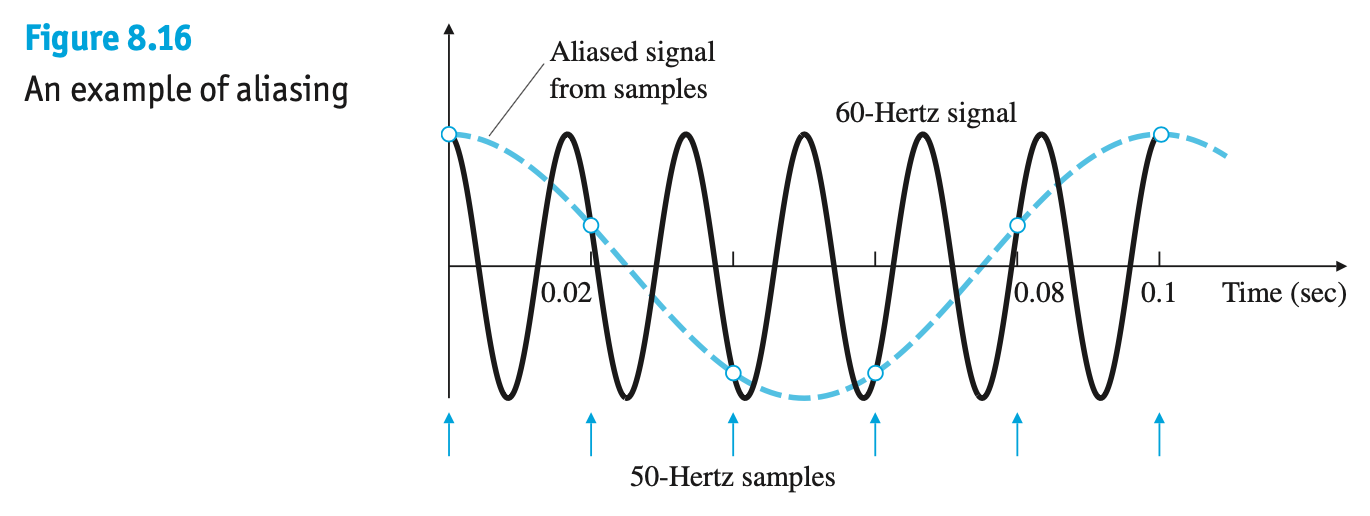
\includegraphics[width=16cm]{./FIG_Franklin_Next/fig8-16.png}
		\end{figure}
		%
		\item Its function is to reduce the higher frequency noise components in the analog signal in order to prevent \emph{aliasing}.
		\item Aliasing will occur any time the sample rate is not at least twice as fast as any of the frequencies in the signal being sampled. 
		\item To prevent aliasing of a 60Hz signal, the sample rate would have to be faster than 120Hz. 
%
\newpage
%
		\item Aliasing can be explained from the \emph{sampling theorem} of Nyquist and Shannon. For the signal to be reconstructed from the samples, it must have no frequency component greater than half the sample rate (\emph{Nyquist rate} of $\omega_s/2$).  
		\item In a continuous system, noise components with a frequency much higher than the control-system bandwidth normally have a small effect because the system will not respond at the high frequency. 
		\item However, in a \emph{digital system}, the frequency of the noise can be \emph{aliased down}  to the vincinity of the system bandwidth so the closed-loop system would respond to the noise.
		\item The solution to prevent aliasing is to place an analog prefilter before the sampler. In many cases, a simple first-order low-pass filter will do - that is - 
		\begin{align*}
			H_p(s) = \frac{a}{s+a}
		\end{align*}
		where the \emph{breakpoint} $a$ is selected to be lower than Nyquist rate $\omega_s/2$ so that any noise present with frequencies greater than Nyquist rate is attenuated by the prefilter. 
		\item If $\omega_s$ is chosen to be $25 \times \omega_{bd}$, the anti-aliasing filter breakpoint $a$ should be selected lower than $\omega_s/2$, so that 
		\begin{align*}
			a = 10 \times \omega_{bd} ~~~~\leftarrow~~~~ \omega_s = 25 \times \omega_{bd} 
		\end{align*}
		would be a reasonable choice. 
	\end{itemize}
\end{itemize}
%
%
\newpage
%
\section{Sample-Rate Selection}
%
\begin{itemize}
	\item The inherent approximation for the discrete TF may give rise to \emph{decreased performance} or even \emph{system instability} as the sample rate is lowered. This can lead the designer to conclude that a faster sample rate is required. 
	\item The \emph{sampling theorem} states that in order to reconstruct an unknown, band-limited, continuous signal from samples of that signal, we must \emph{sample at least twice as fast as the highest frequency contained in the signal}. $\omega_s = 2 \omega_{bd}$  
	\item In the $z$-plane, the highest frequency that can be represented by a discrete system is $\omega_s/2$. 
	\item For a very high frequency noise, it would be foolish to sample fast enough to attenuate the disturbance without the use of a prefilter. 
\end{itemize}
%
%
\newpage
%
\section{Discrete Design} 
%
\begin{itemize}
	\item This plant model can be used as part of a discrete model of the feedback system including the compensation $D_d(z)$. 
	\item Analysis and design using this discrete model is called \emph{discrete design} or alternatively, \emph{direct digital design}. 
	\item For a plant described by $G(s)$ and preceeded by a ZOH, the discrete TF was essentially given by 
	\begin{align*}
		G(z) = (1-z^{-1}) \mathcal{Z} \left\{ \frac{G(s)}{s} \right\}
	\end{align*}
	\begin{figure}[h]
		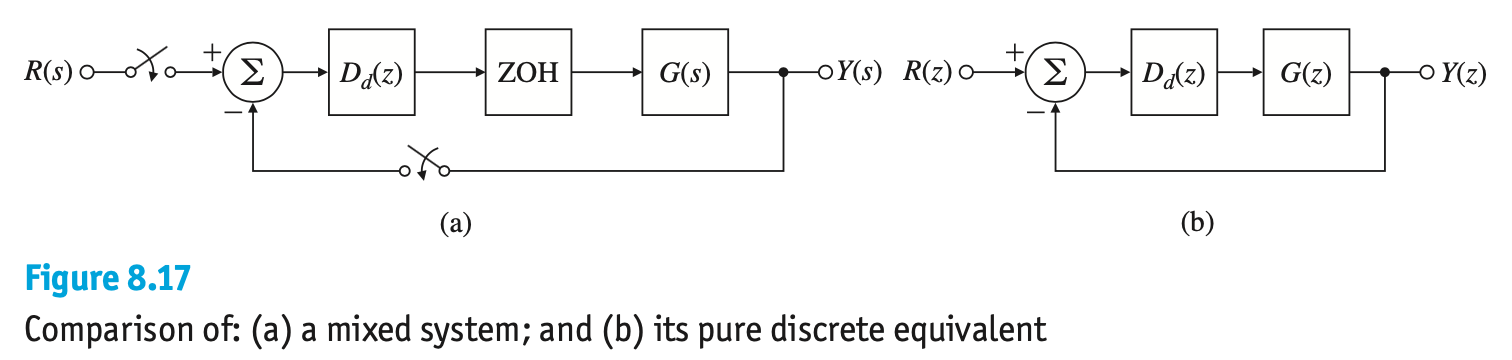
\includegraphics[width=12cm]{./FIG_Franklin_Next/fig8-17.png}
	\end{figure}
	\item The closed-loop poles or the roots of the discrete characteristic equation
	\begin{align*}
		1+ D_d(z) G(z) = 0 
	\end{align*}
	\item The root-locus techniques used in continuous systems to find roots of a polynomial in $s$ apply equally well and without modification to the polynoimal in $z$.
	\item The interpretation of the results is that the stability boundary is now the unit circle instead of the imaginary axis. 
%
\end{itemize}
%

(Example 8.4)  When $G(s) = \frac{a}{s+a}$ and $D_d(z) = K$, draw the root locus with respect to $K$? 

(Answer) 
\begin{align*}
	G(z) &= (1-z^{-1}) \mathcal{Z} \left\{ \frac{a}{s(s+a)} \right\} = (1-z^{-1}) \mathcal{Z} \left\{ \frac{1}{s}  - \frac{1}{s+a} \right\} \\
	&= (1-z^{-1}) \left( \frac{1}{1-z^{-1}} - \frac{1}{1-e^{-aT}z^{-1}} \right)  \\
	&= \frac{(1-e^{-aT})z^{-1}}{1-e^{-aT}z^{-1}} \\
	&= \frac{(1-\alpha)z^{-1}}{1-\alpha z^{-1}} ~~~~~~~\mbox{where}~~ \alpha = e^{-aT}
\end{align*}
The discrete characteristic equation becomes
\begin{align*}
	1+ D_d(z) G(z) = 1 + K\frac{(1-\alpha)z^{-1}}{1-\alpha z^{-1}}= 0 
\end{align*}

\begin{figure}[h]
	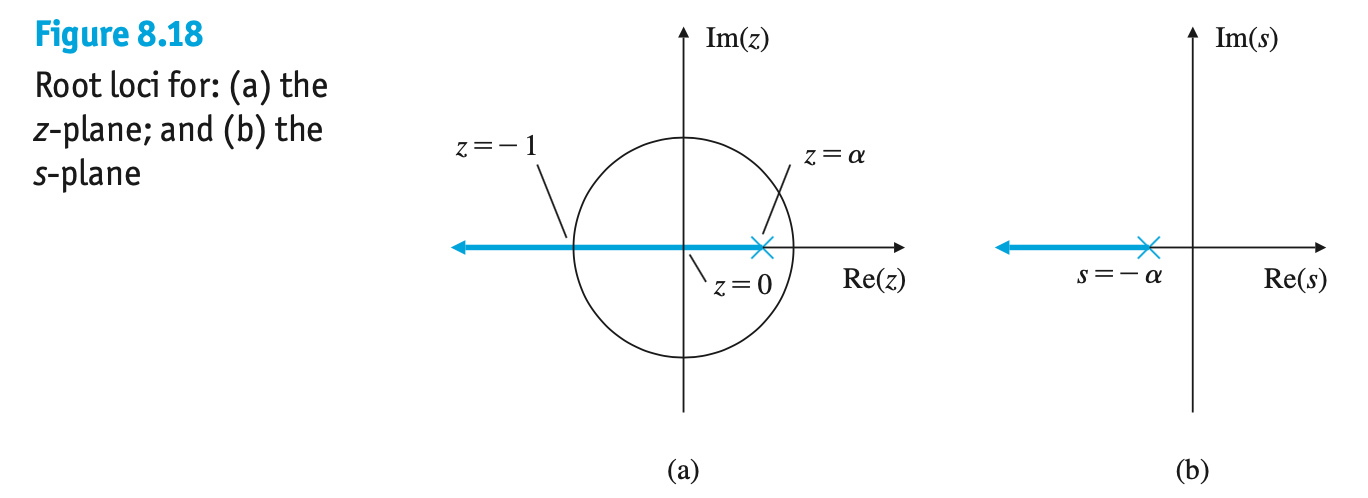
\includegraphics[width=12cm]{./FIG_Franklin_Next/fig8-18.png}
\end{figure}

In the continuous case, the system remains stable for all values of $K$. 
In the discrete case, the system becomes oscillatory with decreasing damping ratio as $z$ goes from 0 to -1 and eventually becomes unstable. This instability is due to the lagging effect of the ZOH. 

%
\newpage
%
Feedback properties 
\begin{itemize}
	\item Proportional 
	\begin{align*}
		u(k) = Ke(k) ~~~~\leftrightarrow~~~~ D_d(z) = K 
	\end{align*}
	\item Derivative 
	\begin{align*}
		u(k) = K T_D [e(k) - e(k-1)] ~~~~~\leftrightarrow~~~~ D_d(z) = KT_D (1-z^{-1})
	\end{align*}
	\item Integral 
	\begin{align*}
		u(k) = u(k-1) + \frac{K}{T_I} e(k) ~~~~~\leftrightarrow~~~~ D_d(z) = \frac{K}{T_I} \left( \frac{1}{1-z^{-1}} \right) 
	\end{align*}
	\item Lead 
	\begin{align*}
		u(k) = \beta u(k-1) + K [e(k) - \alpha e(k-1)] ~~~~~\leftrightarrow~~~~ D_d(z) = K \frac{1- \alpha z^{-1}}{1-\beta z^{-1}} 
	\end{align*}
\end{itemize}
%
%
\newpage
%
%
\newpage
%
(Example 8.5)  Design a digital controller to have a closed-loop natural frequency $\omega_n = 0.3$ and a damping ratio $\zeta = 0.7$ using discrete design

(Answer) 
\begin{align*}
	G(s) = \frac{1}{s^2}   ~~~~~\rightarrow~~~~~~ G(z) = (1-z^{-1}) \mathcal{Z} \left\{ \frac{1}{s^3} \right\} = \frac{T^2}{2} \frac{z^{-1}(1+z^{-1})}{(1-z^{-1})^2}
\end{align*}
which, with $T=1$, becomes
\begin{align*}
	G(z) = \frac{1}{2} \frac{z^{-1}(1+z^{-1})}{(1-z^{-1})^2}
\end{align*}
Let us assume that the PD compensator is used
\begin{align*}
	D_d(z) = K (1- \alpha z^{-1})
\end{align*}
The desired pole locations of $\omega_n = 0.3$ and $\zeta = 0.7$ become $z=0.78 \pm 0.18j$ 
\begin{align*}
	1 + D_d(z) G(z) = 1 + K\frac{1}{2} \frac{z^{-1}(1+z^{-1})(1- \alpha z^{-1})}{(1-z^{-1})^2} =0 
\end{align*}
Now we have 
\begin{align*}
	\alpha = 0.85 ~~~~~~~~~~K = 0.374
\end{align*}
and 
\begin{align*}
	D_d(z) = 0.374 (1- 0.85 z^{-1})
\end{align*}
The difference equation becomes
\begin{align*}
	u(k) =  0.374 [e(k) - 0.85 e(k-1)] 
\end{align*}

(8장 숙제) 8장 연습문제에서 기말고사에 출제될 만한 문제 3개를 선택하여 풀어 제출하라? (마감 기말고사 전) 
% 
\newpage


\end{document}
